
\subsubsection*{Random Exploration}
\label{sec:findings-expts-rand}

%%%
While analysis was being performed on the results of Round 2 and further
experimentation was underway,
the discovery was made that the method for deciding which combination of cards
should be picked was not as expected,
thanks to a overlooking the matter during development.
%
% TODO(Chelsea): reword to make sure tenses agree, kind of disagree
A ``correct'' method of choosing cards would have selected the card combination
corresponding to the maximum value found in the produced $p$ vector,
breaking ties randomly,
with a chance of making an exploration step by selecting a combination at
uniform random.
%
The implemented mechanism did indeed normally choose the maximally represented
combination in the $p$ vector,
but random exploration was performed using the $p$ vector as a probability
distribution.
%
Further complicating the issue,
a review of the code was misunderstood and it was wrongly concluded that
the $p$ vector was normally used as a probability distribution
and random exploration was carried out at uniform.
%%%

%%%
Thanks to the nature of the produced $p$ vectors,
it was assumed that the implemented solution would not make make a marked
difference in performance or learning.
%
This is because $p$ for locations which were untrained 
ended up producing $p$ vectors which were remarkably close to
uniform themselves.
%
However,
states which were trained often produced $p$ vectors in which
three or four combinations of cards were almost equally highly weighted
while unpopular combinations had nearly zero chance of being chosen.
%
While this resulting $p$ vector was created exactly as intended,
the skewing towards certain combinations means that so-called
random exploration steps are unlikely to actually explore policy options
which have no recent bias
in later, trained states.
%
This may result in only a negligible effect since
only highly trained locations will show this bias
and may even be helpful as it allows a set of weights to converge more quickly
to a stable policy.
%%%


\paragraph*{Results}
\label{sec:findings-expts-rand-results}

%%%
% Results of the given experimental change(s) as they are generated.
%%%

%%%
By comparing the strategy graphs created from using the correct selection
methodology seen in Figure~\ref{fig:expts-rand-strats}
to those previously created with the faulty mechanism as in Round 2
such as in Figure~\ref{fig:r2-strats-loser},
it is evident that there is no functional difference between these two
randomization techniques.
%
As expected,
the nature of the produced $p$ vectors lent themselves to nearly uniform random
choice for untrained sets leading to no significant change in exploration in
early game situations.
%
Furthermore,
in trained sets,
the choice between three or four best combinations of cards rather than
the full fifteen possibilities did not negatively affect the learning of
strategy combinations overall.
%%%



\begin{figure}
\center

	\begin{subfigure}[t]{0.22\textwidth}
		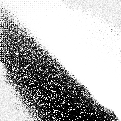
\includegraphics[width=\textwidth]{images/findings/experiments/randomization/strats/hand_max_min.png}
		\caption{\handmaxmin}
	\end{subfigure}
	~
	\begin{subfigure}[t]{0.22\textwidth}
		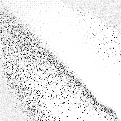
\includegraphics[width=\textwidth]{images/findings/experiments/randomization/strats/hand_max_avg.png}
		\caption{\handmaxavg}
	\end{subfigure}
	~
	\begin{subfigure}[t]{0.22\textwidth}
		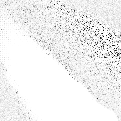
\includegraphics[width=\textwidth]{images/findings/experiments/randomization/strats/hand_max_med.png}
		\caption{\handmaxmed}
	\end{subfigure}
	~
	\begin{subfigure}[t]{0.22\textwidth}
		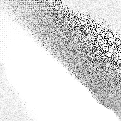
\includegraphics[width=\textwidth]{images/findings/experiments/randomization/strats/hand_max_poss.png}
		\caption{\handmaxposs}
	\end{subfigure}

	\begin{subfigure}[t]{0.22\textwidth}
		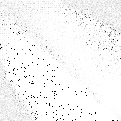
\includegraphics[width=\textwidth]{images/findings/experiments/randomization/strats/crib_min_avg.png}
		\caption{\cribminavg}
	\end{subfigure}
	~
	\begin{subfigure}[t]{0.22\textwidth}
		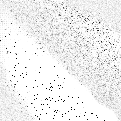
\includegraphics[width=\textwidth]{images/findings/experiments/randomization/strats/pegging_max_avg_gained.png}
		\caption{\peggingmaxavggained}
	\end{subfigure}
	~
	\begin{subfigure}[t]{0.22\textwidth}
		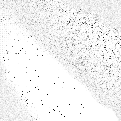
\includegraphics[width=\textwidth]{images/findings/experiments/randomization/strats/pegging_max_med_gained.png}
		\caption{\peggingmaxmedgained}
	\end{subfigure}
	~
	\begin{subfigure}[t]{0.22\textwidth}
		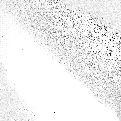
\includegraphics[width=\textwidth]{images/findings/experiments/randomization/strats/pegging_min_avg_given.png}
		\caption{\peggingminavggiven}
	\end{subfigure}

\caption{
	All final strategies for an agent which had its randomization strategy fixed
	to choose the combination of cards corresponding to the maximum value in
	the \pvec\ vector and with a chance of selecting at uniform random.
	These graphs are for when the agent is playing as the dealer.
}
\label{fig:expts-rand-strats}
\end{figure}

%\label{fig:expts-rand-strats}
